\providecommand{\main}{../../../..}

\documentclass[../../../../thesis]{subfiles}


\begin{document}

\section{Module Parser \& Scanner}\label{parser-scanner-module}


%----------------------------------------------------------------------------------------
%	4.3.1: ComicParser
%----------------------------------------------------------------------------------------

\subsection{\texttt{ComicParser}}

\texttt{ComicParser} là một trong các thành phần trung tâm của yacv. Lớp này
nhận vào URI trỏ đến một tệp truyện, và đọc nội dung tệp truyện đó ra. Cần gọi
đủ tên là \texttt{ComicParser}, vì phải phân biệt với hai parser (bộ đọc/giải
mã) khác nhưng tích hợp trong nó:

\begin{table}[H]
    \centering
    \caption{Hai kiểu parser trong \texttt{ComicParser}}
    \label{tab:2-parsers}
    \begin{tabular}{l p{6cm} l}
        \toprule
                & Parser cho tệp nén & Parser cho metadata \\
        \midrule
        Đầu vào & Tệp nén            & Tệp metadata \\
        Đầu ra  & Các tệp con hoặc tương đương (\texttt{InputStream},\ldots) & Đối tượng \texttt{Comic} \\
        \bottomrule
    \end{tabular}
\end{table}

\texttt{ComicParser} được thiết kế theo kiểu ``lười'', có nghĩa là không có
thông tin nào được đọc ra cho đến khi thực sự cần. Lý do vẫn là vấn đề về hiệu
năng, vì gần như mọi thao tác đọc trong SAF - hệ thống đọc ghi tệp của Android -
đều rất chậm.

\subsubsection{Parser cho tệp nén}

Parser cho tệp nén hiện gồm một giao diện và hai lớp:

\begin{itemize}
    \item
        \texttt{ArchiveParser}: giao diện chung cho mọi parser tệp nén
    \item
        \texttt{CBZParser}: parser riêng cho tệp CBZ
    \item
        \texttt{ArchiveParserFactory}: giúp khởi tạo các parser
\end{itemize}

\texttt{ArchiveParser} là một giao diện (interface), định nghĩa một số phương
thức chung mọi parser cho tệp nén đều phải có. Do hiện tại yacv mới hỗ trợ định
dạng CBZ, chỉ có lớp \texttt{CBZParser} cài đặt giao diện này.

Trong \texttt{ArchiveParser}, có hai phương thức quan trọng:

\begin{itemize}
    \item
        \texttt{getEntryOffsets()}: Phương thức này trả về một từ điển như sau:

        \begin{itemize}
            \item
                Khóa: tên tệp lẻ
            \item
                Giá trị: offset tệp lẻ, tức vị trí tệp lẻ trong tệp nén
        \end{itemize}
    \item
        \texttt{readEntryAtOffset()}: Phương thức này nhận vào một offset, và
        trả về \texttt{InputStream} tương ứng với tệp lẻ ở offset đó bằng cách
        ``nhảy cóc'' đến đúng chỗ và đọc.
\end{itemize}

\texttt{ArchiveParserFactory} là một lớp theo mẫu thiết kế factory, nhận
vào URI của tệp truyện và trả về \texttt{ArchiveParser} để đọc loại tệp truyện
đó (ví dụ, nếu URI có đuôi CBZ thì trả về một đối tượng \texttt{CBZParser}). Do
\texttt{ArchiveParser} cần một số cài đặt khởi tạo riêng, nên mới cần một lớp
riêng để tạo parser. Chữ ``Factory'' thể hiện lớp này sử dụng mẫu thiết kế
factory.

\subsubsection{Parser cho metadata}

yacv hiện hỗ trợ định dạng ComicRack, được giới thiệu chi tiết trong Phụ lục 2.
Định dạng này là một tệp tin XML, do đó được đọc đơn giản bằng các thư viện XML
sẵn có.

Để mở rộng định dạng tệp đọc, có thể dùng mẫu thiết kế factory như đã dùng với
parser cho tệp. Theo cách này, các parser cần có hàm \texttt{parse()} trả về một
đối tượng \texttt{Comic} và nhận hai tham số:

\begin{itemize}
    \item
        Nội dung tệp metadata: ở dạng chuỗi thông thường
    \item
        Tên tệp metadata: tên tệp giúp phân biệt các định dạng tệp với nhau
\end{itemize}


%----------------------------------------------------------------------------------------
%	4.3.2: CBZParser
%----------------------------------------------------------------------------------------

\subsection{\texttt{CBZParser}}

\texttt{CBZParser} là lớp cài đặt giao diện \texttt{ArchiveParser}. Như đã phân
tích ở Chương 2, hệ thống đọc ghi tệp SAF của Android chỉ cho phép đọc ghi tuần
tự. Việc tạo ra mảng offset không đơn giản, do phần mục lục của tệp ZIP nằm ở
cuối, và có nhiều thao tác cần dò ngược từ cuối lên.

Để giải quyết vấn đề danh sách offset, có hai cách đơn giản nhất:

\begin{itemize}
    \item
        Chép toàn bộ tệp truyện vào phần bộ nhớ riêng của ứng dụng

        \begin{itemize}
            \item
                Ưu: Phần bộ nhớ này vẫn được dùng API File của Java, do đó có
                thể đọc ghi ngẫu nhiên, cho phép đọc mục lục rất nhanh.
            \item
                Nhược: Tệp truyện rất nặng (vài chục đến vài trăm MB) dẫn đến
                tốn cả dung lượng đĩa lẫn băng thông đọc/ghi. Ghi xóa liên tục
                cũng có hại cho bộ nhớ thể rắn của điện thoại.
        \end{itemize}
    \item
        Đọc tệp ZIP ở chế độ đọc tuần tự

        \begin{itemize}
            \item
                Ưu: Dùng ngay được với cơ chế đọc qua \texttt{InputStream} của
                SAF
            \item
                Nhược: Do không có mục lục, dữ liệu phải được ``dò'' từ từ để
                đọc từng tệp lẻ một. Hậu quả là phương pháp này vừa tốn băng
                thông đọc, vừa tốn CPU để giải nén những tệp không cần thiết.
        \end{itemize}
\end{itemize}

\texttt{CBZParse} giải quyết vấn đề này bằng cách làm giả một luồng nhập ngẫu
nhiên, sẽ được miêu tả rõ hơn trong \autoref{sec:cbzparser}. Cách làm đó có thể
được tóm tắt như sau:

\begin{itemize}
    \item
        Hai phần đầu tệp nén được lưu đệm trong RAM, do là hai phần có nhiều
        truy cập nhất trong khi đọc mục lục
    \item
        Các phần còn lại được đọc xuôi khi cần theo luồng nhập
        \texttt{InputStream}, nếu đọc ngược sẽ phải tạo mới luồng nhập
\end{itemize}

Kết quả là mục lục đọc được mà chỉ cần:

\begin{itemize}
    \item
        Trung bình hai lần đọc tuần tự theo \texttt{InputStream}
    \item
        Không phải ghi ra đĩa
    \item
        Không phải giải nén những tệp không cần thiết
\end{itemize}


%----------------------------------------------------------------------------------------
%	4.3.3: Tổng hợp lại ComicParser
%----------------------------------------------------------------------------------------

\subsection{Tổng hợp lại \texttt{ComicParser}}

Tương tác trong một ca sử dụng hiển thị của \texttt{ComicParser} được mô tả
trong \autoref{fig:parser_sequence}.

Nhắc lại rằng do metadata không chỉ định, thứ tự trang truyện chỉ có thể suy ra
từ thứ tự tên tệp ảnh. Không có quy chuẩn cho tên trang truyện, tuy nhiên đa số
các tệp truyện đặt tên theo định dạng sau:

\begin{verbatim}
X-Men Vol 40 1.jpg
│     │      └─ Trang truyện số
│     └─ Số Volume, Number,...
└─ Tên tệp truyện
\end{verbatim}

Vấn đề với định dạng này xuất hiện khi truyện có nhiều hơn 10 trang. Khi sắp xếp
tệp ảnh theo ABC, các trang sẽ có thứ tự như sau:

\begin{verbatim}
X-Men Vol 40 1.jpg
X-Men Vol 40 10.jpg
X-Men Vol 40 11.jpg
...
X-Men Vol 40 19.jpg
X-Men Vol 40 2.jpg
...
\end{verbatim}

Ta thấy ngay rằng thứ tự tệp ảnh trang truyện bị đảo lộn. Để giải quyết vấn đề
này, cần viết hàm so sánh riêng cho tên tệp ảnh. Ý tưởng ở đây là gom những kí
tự số liên tiếp với nhau thành một ``kí tự'' rồi mới so sánh. Đoạn mã giả sau
đây trình bày thuật toán:

\begin{Verbatim}[samepage=true]
def compare(str1, str2):
    arrs = []

    for str in [str1, str2]:
        arrtmp = []
        acc = []

        for char in str:
            if is_number(char):
                acc.append(char)
            else:
                if len(acc) != 0:
                    acc = ''.join(acc)
                    acc = to_num(acc)
                    arrtmp.append(acc)
                    acc = 0
                arrtmp.append(to_codepoint(char))

    return compare_left_to_right(arrs[0], arrs[1])
\end{Verbatim}

\begin{figure}[H]
    \centering
    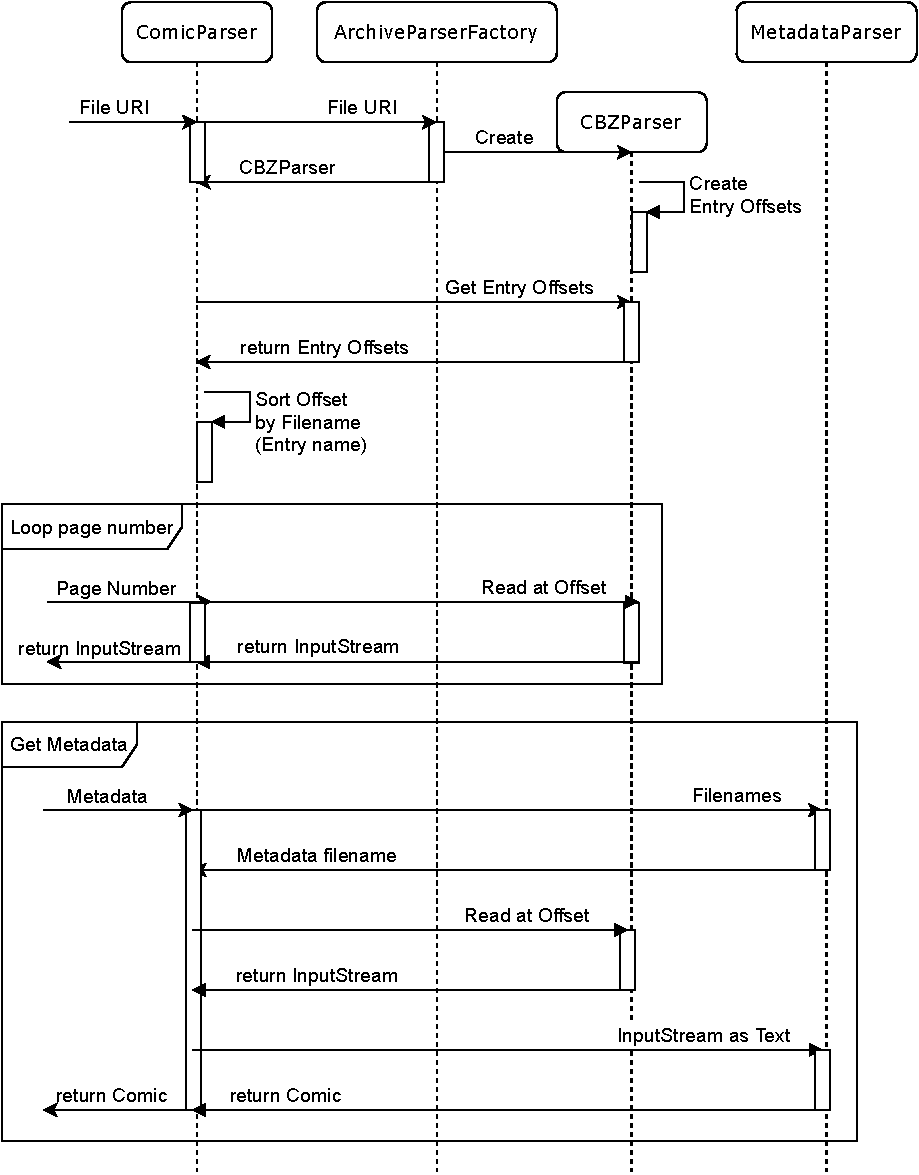
\includegraphics[scale=0.8]{../images/parser_sequence.pdf}
    \caption{\texttt{ComicParser} và các thành phần của nó}
    \label{fig:parser_sequence}
\end{figure}


%----------------------------------------------------------------------------------------
%	4.3.4: Scanner
%----------------------------------------------------------------------------------------

\subsubsection{Scanner}

Đây là lớp phục vụ cho tính năng quét truyện trong yacv. Biểu đồ luồng của ca sử
dụng \emph{quét mới} được thể hiện trong \autoref{fig:scan_new_sequence}.

\begin{figure}[H]
    \centering
    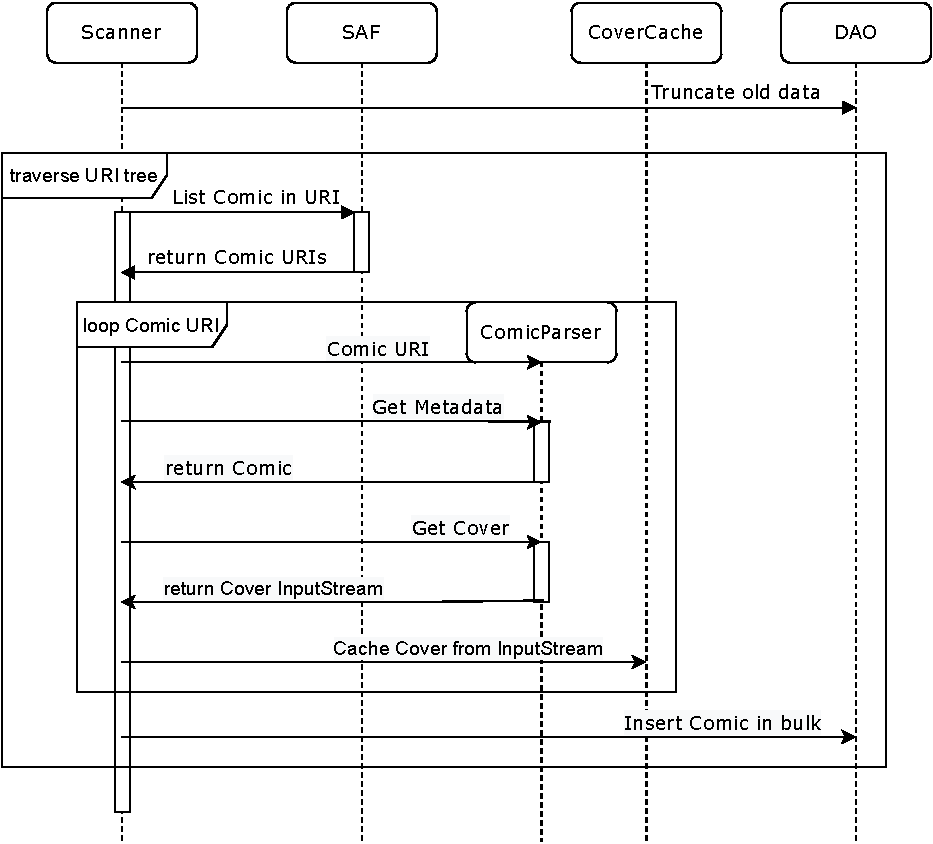
\includegraphics[scale=0.8]{../images/scan_new_sequence.pdf}
    \caption{Biểu đồ tuần tự của ca sử dụng quét mới tệp truyện}
    \label{fig:scan_new_sequence}
\end{figure}

Một chi tiết mới trong biểu đồ này là lớp \texttt{ImageCache}, sẽ được giới
thiệu ở mục về cache ảnh.

Ca sử dụng quét lại cũng có thiết kế gần tương tự, trong đó bỏ bước xóa dữ liệu,
và thêm một bước quét cơ sở dữ liệu sau cùng để xóa truyện không còn trong bộ
nhớ. Việc cập nhật và thêm truyện mới được thực hiện trong vòng lặp lớn bình
thường.

Scanner nhận vào URI của thư mục gốc, rồi lặp qua từng tệp con, cháu,\ldots{}
Nếu đó là tệp truyện, nó gọi `ComicParser' để lấy metadata, rồi lưu vào cơ sở dữ
liệu qua DAO.

Quá trình quét tệp này giống như duyệt cây, do đó có hai cách cơ bản:

\begin{itemize}
    \item
        Duyệt theo độ sâu (depth-first search, gọi tắt là DFS)
    \item
        Duyệt theo độ rộng (breadth-first search, gọi tắt là BFS)
\end{itemize}

Trong trường hợp cụ thể này, DFS được chọn. Lý do cho lựa chọn này là DFS có thể
phát hiện \emph{thư mục} nhanh hơn nhiều so với BFS. Mỗi khi gặp thư mục, DFS xử
lí (thêm vào cơ sở dữ liệu) ngay, thay vì thêm vào hàng đợi. Do phát hiện được
thư mục nhanh hơn BFS, Màn hình Thư viện, vốn hiển thị danh sách các \emph{thư
mục}, cũng hiển thị sớm hơn. Dù thời gian quét tổng thể không thay đổi, người
dùng được thấy thư mục sớm hơn giúp tạo cảm giác ứng dụng khá nhanh.

\end{document}
